
\documentclass[a4paper,11pt]{article}
\usepackage[a4paper, margin=8em]{geometry}

% usa i pacchetti per la scrittura in italiano
\usepackage[french,italian]{babel}
\usepackage[T1]{fontenc}
\usepackage[utf8]{inputenc}
\frenchspacing 

% usa i pacchetti per la formattazione matematica
\usepackage{amsmath, amssymb, amsthm, amsfonts}

% usa altri pacchetti
\usepackage{gensymb}
\usepackage{hyperref}
\usepackage{standalone}

\usepackage{colortbl}

\usepackage{xstring}
\usepackage{karnaugh-map}

% imposta il titolo
\title{Appunti Calcolatori Elettronici}
\author{Luca Seggiani}
\date{2025}

% imposta lo stile
% usa helvetica
\usepackage[scaled]{helvet}
% usa palatin
\usepackage{palatino}
% usa un font monospazio guardabile
\usepackage{lmodern}

\renewcommand{\rmdefault}{ppl}
\renewcommand{\sfdefault}{phv}
\renewcommand{\ttdefault}{lmtt}

% circuiti
\usepackage{circuitikz}
\usetikzlibrary{babel}

% testo cerchiato
\newcommand*\circled[1]{\tikz[baseline=(char.base)]{
            \node[shape=circle,draw,inner sep=2pt] (char) {#1};}}

% disponi il titolo
\makeatletter
\renewcommand{\maketitle} {
	\begin{center} 
		\begin{minipage}[t]{.8\textwidth}
			\textsf{\huge\bfseries \@title} 
		\end{minipage}%
		\begin{minipage}[t]{.2\textwidth}
			\raggedleft \vspace{-1.65em}
			\textsf{\small \@author} \vfill
			\textsf{\small \@date}
		\end{minipage}
		\par
	\end{center}

	\thispagestyle{empty}
	\pagestyle{fancy}
}
\makeatother

% disponi teoremi
\usepackage{tcolorbox}
\newtcolorbox[auto counter, number within=section]{theorem}[2][]{%
	colback=blue!10, 
	colframe=blue!40!black, 
	sharp corners=northwest,
	fonttitle=\sffamily\bfseries, 
	title=Teorema~\thetcbcounter: #2, 
	#1
}

% disponi definizioni
\newtcolorbox[auto counter, number within=section]{definition}[2][]{%
	colback=red!10,
	colframe=red!40!black,
	sharp corners=northwest,
	fonttitle=\sffamily\bfseries,
	title=Definizione~\thetcbcounter: #2,
	#1
}

% disponi codice
\usepackage{listings}
\usepackage[table]{xcolor}

\definecolor{codegreen}{rgb}{0,0.6,0}
\definecolor{codegray}{rgb}{0.5,0.5,0.5}
\definecolor{codepurple}{rgb}{0.58,0,0.82}
\definecolor{backcolour}{rgb}{0.95,0.95,0.92}

\lstdefinestyle{codestyle}{
		backgroundcolor=\color{black!5}, 
		commentstyle=\color{codegreen},
		keywordstyle=\bfseries\color{magenta},
		numberstyle=\sffamily\tiny\color{black!60},
		stringstyle=\color{green!50!black},
		basicstyle=\ttfamily\footnotesize,
		breakatwhitespace=false,         
		breaklines=true,                 
		captionpos=b,                    
		keepspaces=true,                 
		numbers=left,                    
		numbersep=5pt,                  
		showspaces=false,                
		showstringspaces=false,
		showtabs=false,                  
		tabsize=2
}

\lstdefinestyle{shellstyle}{
		backgroundcolor=\color{black!5}, 
		basicstyle=\ttfamily\footnotesize\color{black}, 
		commentstyle=\color{black}, 
		keywordstyle=\color{black},
		numberstyle=\color{black!5},
		stringstyle=\color{black}, 
		showspaces=false,
		showstringspaces=false, 
		showtabs=false, 
		tabsize=2, 
		numbers=none, 
		breaklines=true
}


\lstdefinelanguage{assembler}{ 
  keywords={AAA, AAD, AAM, AAS, ADC, ADCB, ADCW, ADCL, ADD, ADDB, ADDW, ADDL, AND, ANDB, ANDW, ANDL,
        ARPL, BOUND, BSF, BSFL, BSFW, BSR, BSRL, BSRW, BSWAP, BT, BTC, BTCB, BTCW, BTCL, BTR, 
        BTRB, BTRW, BTRL, BTS, BTSB, BTSW, BTSL, CALL, CBW, CDQ, CLC, CLD, CLI, CLTS, CMC, CMP,
        CMPB, CMPW, CMPL, CMPS, CMPSB, CMPSD, CMPSW, CMPXCHG, CMPXCHGB, CMPXCHGW, CMPXCHGL,
        CMPXCHG8B, CPUID, CWDE, DAA, DAS, DEC, DECB, DECW, DECL, DIV, DIVB, DIVW, DIVL, ENTER,
        HLT, IDIV, IDIVB, IDIVW, IDIVL, IMUL, IMULB, IMULW, IMULL, IN, INB, INW, INL, INC, INCB,
        INCW, INCL, INS, INSB, INSD, INSW, INT, INT3, INTO, INVD, INVLPG, IRET, IRETD, JA, JAE,
        JB, JBE, JC, JCXZ, JE, JECXZ, JG, JGE, JL, JLE, JMP, JNA, JNAE, JNB, JNBE, JNC, JNE, JNG,
        JNGE, JNL, JNLE, JNO, JNP, JNS, JNZ, JO, JP, JPE, JPO, JS, JZ, LAHF, LAR, LCALL, LDS,
        LEA, LEAVE, LES, LFS, LGDT, LGS, LIDT, LMSW, LOCK, LODSB, LODSD, LODSW, LOOP, LOOPE,
        LOOPNE, LSL, LSS, LTR, MOV, MOVB, MOVW, MOVL, MOVSB, MOVSD, MOVSW, MOVSX, MOVSXB,
        MOVSXW, MOVSXL, MOVZX, MOVZXB, MOVZXW, MOVZXL, MUL, MULB, MULW, MULL, NEG, NEGB, NEGW,
        NEGL, NOP, NOT, NOTB, NOTW, NOTL, OR, ORB, ORW, ORL, OUT, OUTB, OUTW, OUTL, OUTSB, OUTSD,
        OUTSW, POP, POPL, POPW, POPB, POPA, POPAD, POPF, POPFD, PUSH, PUSHL, PUSHW, PUSHB, PUSHA, 
				PUSHAD, PUSHF, PUSHFD, RCL, RCLB, RCLW, MOVSL, MOVSB, MOVSW, STOSL, STOSB, STOSW, LODSB, LODSW,
				LODSL, INSB, INSW, INSL, OUTSB, OUTSL, OUTSW
        RCLL, RCR, RCRB, RCRW, RCRL, RDMSR, RDPMC, RDTSC, REP, REPE, REPNE, RET, ROL, ROLB, ROLW,
        ROLL, ROR, RORB, RORW, RORL, SAHF, SAL, SALB, SALW, SALL, SAR, SARB, SARW, SARL, SBB,
        SBBB, SBBW, SBBL, SCASB, SCASD, SCASW, SETA, SETAE, SETB, SETBE, SETC, SETE, SETG, SETGE,
        SETL, SETLE, SETNA, SETNAE, SETNB, SETNBE, SETNC, SETNE, SETNG, SETNGE, SETNL, SETNLE,
        SETNO, SETNP, SETNS, SETNZ, SETO, SETP, SETPE, SETPO, SETS, SETZ, SGDT, SHL, SHLB, SHLW,
        SHLL, SHLD, SHR, SHRB, SHRW, SHRL, SHRD, SIDT, SLDT, SMSW, STC, STD, STI, STOSB, STOSD,
        STOSW, STR, SUB, SUBB, SUBW, SUBL, TEST, TESTB, TESTW, TESTL, VERR, VERW, WAIT, WBINVD,
        XADD, XADDB, XADDW, XADDL, XCHG, XCHGB, XCHGW, XCHGL, XLAT, XLATB, XOR, XORB, XORW, XORL},
  keywordstyle=\color{blue}\bfseries,
  ndkeywordstyle=\color{darkgray}\bfseries,
  identifierstyle=\color{black},
  sensitive=false,
  comment=[l]{\#},
  morecomment=[s]{/*}{*/},
  commentstyle=\color{purple}\ttfamily,
  stringstyle=\color{red}\ttfamily,
  morestring=[b]',
  morestring=[b]"
}

\lstset{language=assembler, style=codestyle}

% disponi sezioni
\usepackage{titlesec}

\titleformat{\section}
	{\sffamily\Large\bfseries} 
	{\thesection}{1em}{} 
\titleformat{\subsection}
	{\sffamily\large\bfseries}   
	{\thesubsection}{1em}{} 
\titleformat{\subsubsection}
	{\sffamily\normalsize\bfseries} 
	{\thesubsubsection}{1em}{}

% tikz
\usepackage{tikz}

% float
\usepackage{float}

% grafici
\usepackage{pgfplots}
\pgfplotsset{width=10cm,compat=1.9}

% disponi alberi
\usepackage{forest}

\forestset{
	rectstyle/.style={
		for tree={rectangle,draw,font=\large\sffamily}
	},
	roundstyle/.style={
		for tree={circle,draw,font=\large}
	}
}

% disponi algoritmi
\usepackage{algorithm}
\usepackage{algorithmic}
\makeatletter
\renewcommand{\ALG@name}{Algoritmo}
\makeatother

% disponi numeri di pagina
\usepackage{fancyhdr}
\fancyhf{} 
\fancyfoot[L]{\sffamily{\thepage}}

\makeatletter
\fancyhead[L]{\raisebox{1ex}[0pt][0pt]{\sffamily{\@title \ \@date}}} 
\fancyhead[R]{\raisebox{1ex}[0pt][0pt]{\sffamily{\@author}}}
\makeatother

\begin{document}
% sezione (data)
\section{Lezione del 25-02-25}

% stili pagina
\thispagestyle{empty}
\pagestyle{fancy}

% testo
\subsection{Interazione fra CPU e memoria}
Nell'architettura Intel x86 la CPU interroga la RAM in due situazioni:
\begin{itemize}
	\item Durante la lettura di un istruzione;
	\item Durante la lettura di \textit{eventuali} operandi in memoria richiesti dall'istruzione.
		Notiamo che per ogni istruzione è previsto un solo indirizzo esplicito di un operando in memoria (non è permesso scrivere qualcosa come \lstinline|MOV (%RBP), (%RDI)|). indirizzo
		Alcune istruzioni possono però avere comunque più di un operando in memoria (ad esempio le istruzioni di stringa, \lstinline|MOVS|, ecc... o la stessa istruzione di pila \lstinline|POP|).
\end{itemize}

Dal punto di vista pratico, il collegamento fra CPU e RAM è rappresentato da:
\begin{itemize}
	\item Un \textbf{bus dati} a 64 bit;
	\item Un certo numero di linee per il \textbf{numero di riga}. Questo non corrisponde all'indirizzo del primo byte contenuto in ogni riga, ma l'indice proprio di ogni regione (intesa come riga) da 64 bit all'interno della RAM. Si noti inoltre che queste non sono necessariamente $2^{64}$, o $2^{57}$ (il massimo spazio indirizzabile secondo l'architettura x86), ma più spesso intorno alle $2^{36}$-$2^{37}$;
	\item Determinate \textbf{linee di controllo} che segnalano l'operazione in corso da parte del processore.
	\item 8 linee di \textbf{byte enable}, attive basse, che rappresentano i byte di interesse all'interno di ogni locazione da 64 bit della RAM. Dal punto di vista della lettura, queste linee non sono particolarmente utili in quanto tutta la locazione verrà comunque riportata sul bus dati, o comunque le locazioni non selezionate potranno essere invalide o in alta impedenza, senza avere effetto sulla CPU (che non le leggerà). Per quanto riguarda la scrittura, invece, la RAM lascerà inalterati i byte con byte enable alto. 
\end{itemize}

\subsubsection{Struttura della RAM}
Modelliziamo un modulo di RAM come una rete provvista di:
\begin{itemize}
	\item Una linea di \textbf{select}, attiva bassa;
	\item Le \textbf{linee di indirizzo};
	\item Una linea di \textit{memory read} e una linea di \textit{memory write}, o comunque un certo numero di \textbf{linee di controllo} necessarie all'accesso in scrittura e lettura;
	\item Un \textbf{bus dati} di ingresso/uscita. 
\end{itemize}

Dalla CPU arriveranno, come abbiamo detto, i \textbf{numeri di riga}, i \textbf{byte enable}, il \textbf{bus dati} e le \textbf{linee di controllo}.

I numeri di riga si collegano direttamente alle linee di indirizzo di ogni modulo, che rappresenterà un certo byte della locazione (avremo quindi, nell'architettura descritta, 8 moduli per 8 byte, quindi 64 bit).
I byte enable dovranno quindi smistarsi nelle linee di select di ogni modulo di RAM, a selezionare il modulo corrispondente.
Il bus dati verrà composto, analogamente, concatenando le linee di uscita da 8 bit di ogni modulo di RAM. 
Notiamo che avevamo chiamato questo montaggio \textbf{parallelo}.

\par\smallskip 

Vorremo poter estendere la memoria disponibile oltre il numero di locazioni da un byte fornite da ogni modulo di RAM.
Pensiamo di fare questo attraverso più banchi di memoria con locazioni da 64 bit.
In questo caso avremo bisogno di montaggio in \textbf{serie}, e quindi di generare un segnale di select a partire non solo dalle line di byte enable, ma anche da una \textbf{maschera} generata a partire dal numero di riga.
Questo si potrà fare agevolemnte mettendo il segnale di uscita della maschera in OR (ricordiamo segnali attivi bassi, quindi si applica De Morgan) con il byte enable di ogni modulo di RAM compreso nel banco di memoria associato a tale maschera.

La struttura complessiva della RAM sarà quindi la seguente:
\begin{center}
	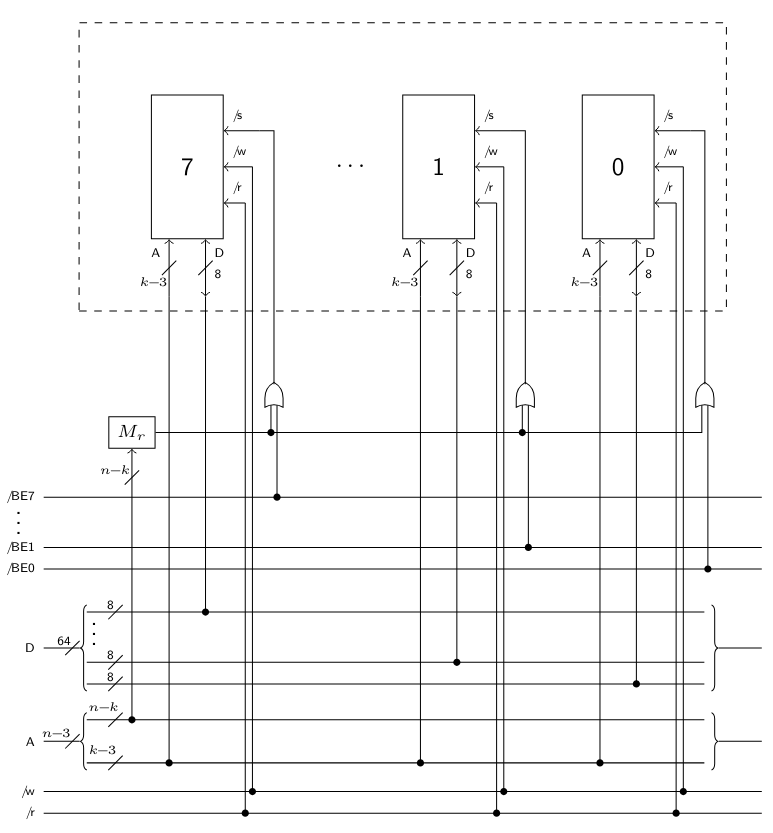
\includegraphics[scale=0.6]{../figures/ram.png}
\end{center}
dove la rete $M_r$ è quella che si occupa di generare la maschera, prendendo banchi di dimensione $2^k$ righe.

\subsubsection{Allineamento e RAM}
Quanto discusso finora rende più chiaro l'importanza del corretto allineamento degli oggetti in memoria.
Leggere un oggetto da 8 byte non allineato nel montaggio di RAM descritto, infatti, richiederà necessariamente 2 accessi, contro il singolo accesso necessario per un oggetto allineato.
Inoltre, alcuni dei byte più significativi risulteranno invertiti di posto rispetto ai byte meno significativi, cioè si richiede un operazione di shift interna al processore.

Questa combinazione di operazioni, eseguite in \textbf{hardware}, rende gli accessi in memoria non allineati molto poco performanti, e quindi sconsigliati (anche se l'architettura Intel x86 li permette comunque).

\par\medskip 

Un problema che potrebbe interessarci è, data una regione di memoria $[x, y)]$ di dimensione $b$ uguale a un singolo banco di RAM, ottenere gli indici della prima regione in cui cade l'intervallo, e la prima in cui non cade più.

Vediamo come calcolare la prima regione di appartenenza.
In \textbf{hardware}, questo può essere calcolato semplicemente prendendo gli $n - b$ bit più significativi dei numeri di riga $x$ e $y$.

In \textbf{software}, questo equivarrà ad uno shift a destra che conservi i soli $n-b$ bit più significativi.

Vediamo come calcolare l'offset di $x$ o $y$ all'interno delle rispettive regioni.
Mascherando gli stessi bit, invece, si può ottenere l'indirizzo all'interno del banco del confine della regione.
Per la precisione, vogliamo una maschera fatta da $n - b$ 0 e $b$ 1.
Questa si può ricavare agevolmente prendendo $2^b$ come \lstinline|1UL << b| e sottrandogli 1, ottenendo la maschera desiderata (si avranno borrow propagati dal bit in $b$ fino al LSB).

Infine, vediamo come calcolare la prima regione di non appartenenza.
In questo caso potremo calcolare la regione in cui cade $y - 1$, e aggiungervi 1 (tenendo conto di eventuali \textit{wrap-around}). Il $-1$ è richiesto dal fatto che $y$ potrebbe cadere sul confine.
In questo caso avremo \lstinline|((y - 1) >> b) + 1|, considerata somma modulo $n - b$.
Alternativamente, si può prendere $y + b$ e calcolarne la regione di appartenenza.

\subsection{Spazio di I/O}
Veniamo quindi alla trattazione dello spazio di I/O e delle interfacce ivi connesse.
L'accesso alle periferiche viene fatto attraverso le istruzioni \lstinline|IN| e \lstinline|OUT|, ammesso che non ci sia nessun sistema operativo in esecuzione, ma solo il nostro programma, e appositi sottoprogrammi di ingresso/uscita, la cui struttura non è al momento importante.

Le periferiche che studieremo, per semplicità di trattazione, derivano in parte da quelle disponibili sui PC \textbf{IBM AT} (famiglia \textit{IBM 5170}).
I PC di questa categoria (compresi tutti i vari \textit{IBM compatible}) si basavano sullo standard per periferiche \textbf{ISA} (\textit{Industry Standard Architecture}).
Visto che i PC moderni derivano dai vecchi IBM compatible, anche oggi si cerca di emulare (almeno in parte) questo standard.

Le periferiche, nello specifico saranno:
\begin{itemize}
	\item La \textbf{tastiera};
	\item Il \textbf{video} su VGA;
	\item Il \textbf{timer};
	\item Gli \textbf{hard disk}.
\end{itemize}

\subsection{Tastiera}
Dal punto di vista funzionale, la tastiera deve solo scoprire quali tasti sono premuti e comunicarlo al calcolatore.
In particolare, noi studieremo tastiere IBM che trasmettono secondo lo standard PS/2.

Nei PC IBM il tasto non restituisce il carattere ASCII del carattere premuto, ma un codice associato ad ogni tasto che va convertito in software.
Questo codice viene ottenuto per \textit{scansione} dell'intero piano della tastiera.
Dal punto di vista meccanico, ci sono \textbf{tracce} orizzontali e verticali disposte, rispettivamente, su ogni riga o colonna di tasti.
La pressione di un tasto comporta una deformazione delle tracce che chiude un circuito fra la riga e la colonna del tasto corrispondente.
Un \textbf{microcontrollore} (originariamente un Intel 8042) collegato sia alle tracce orizzontali che alle tracce verticali scansiona ciclicamente, con impulsi, o le righe leggendo le colonne, o le colonne leggendo rige, cercando un circuito chiuso.
Un cortocircuito viene quindi rilevato dal microcontrollore, che aggiorna una (piccola) memoria interna con il tasto premuto.
Di conseguenza, invia al calcolatore un segnale che codifica quali tasti sono stati premuti rispetto al precedente istante temporale, e quali tasti sono stati rilasciati rispetto al precedente istante temporale. 

La tastiera non restituisce solo pressioni di tasti, ma anche i loro rilasci, cosa che può essere utile per ottenere combinazioni di tasti, pressioni estese nel tempo, ecc...
I codici di pressione si dicono \textbf{make code}, mentre i codici di rilascio si dicono \textbf{break code} 
La stessa pressione ripetuta di un tasto quando l'utente lo tiene premuto per un certo istante temporale era, nei PC IBM, realizzata direttamente nella tastiera (tecnologia \textit{type-matic}), tra l'altro con periodo configurabile.
Tramite il \textit{type-matic}, su appositi tasti abilitati, si ha infatti una ripetizione dell'evento di \textit{pressione} (non rilascio) di un tasto a frequenza costante dopo un intervallo di pressione continua.

Lato calcolatore, il segnale prodotto dal microcontrollore della tastiera viene letto da un interfaccia provvista dei seguenti registri:
\begin{table}[H]
	\center 
	\begin{tabular} { c | p{7cm} }
		\lstinline|0x60| & \textbf{RBR}, \textit{Receive Buffer Register} \\ 
		& \textbf{TBR}, \textit{Transmit Buffer Register} \\ 
		\hline
		... & \\
		\hline
		\lstinline|0x64| & \textbf{STR}, \textit{Status Register} \\
		& \textbf{CMR}, \textit{Command register}
	\end{tabular}
\end{table}

\begin{itemize}
\end{itemize}

RBR e TBR, come STR e CMR, condividono gli indirizzi, rispettivamente \lstinline|0x60| e \lstinline|0x64|.
Il RBR conterrà i make e break code, mentre l'STR conterrà i flag di stato sia per RBR che per TBR (rispettivamente ai bit 0 e 1).

Potremmo chiederci il significato di un registro di trasmissione TBR.
Questo serve, ad esempio, a governare i led di stato per funzioni speciali quali Caps-Lock, Num-Lock, Scroll-Lock ecc... nonché a modificare le impostazioni del \text{type-matic} e, in maniera completamente slegata alla tastiera, a provocare il reset del PC, scrivendo \lstinline|0xFE| in CMR.

Vediamo quindi un programma C++ per l'interazione con l'interfaccia di tastiera.
Notiamo che la libreria all'header \lstinline|libce.h| definisce alcuni tipi (qui \lstinline|natb|, un naturale su 8 bit, e \lstinline|ioaddr|, un indirizzo nello spazio di I/O) e funzioni (qui \lstinline|inputb|, ottieni byte dallo spazio di I/O, e \lstinline|vi::char_write()|, stampa un carattere a schermo).

\lstset{language=C++}
\lstinputlisting{../code/interfaces/keyboard/keyboard.cpp}

Dal programma si evincono subito gli indirizzi dei registri di Receive Buffer (RBR) e di stato (STR), a cui i registri trasmettitore e comando (TBR e CMR) sono sovrapposti.
Il funzionamento è quindi ottenuto attraverso una lettura ciclica dei make code dall'interfaccia, e una scansione per il rilevamento del carattere selezionato a partire dal make code stesso.
Altro codice è usato per gestire il tasto shift, e il termine dell'esecuzione alla pressione del tasto ESC.

\end{document}
